\section{Introduction}
Modern time-series anomaly detection (TSAD) uses increasingly sophisticated detectors, yet simple scorers based on local variation and deviation remain surprisingly competitive~\cite{zhu2026oneliners}. When a complex detector performs well, does it capture anomaly-relevant structure beyond simple statistics, or largely re-express patterns already present in the time series? Benchmarks such as TSB-AD~\cite{liu2024tsbad} characterize standalone detection performance but do not directly answer what a detector adds beyond a statistical reference.

Work on foundation models asks whether learned scores provide value beyond window statistics~\cite{stability2026}. Predictive $\mathcal V$-information studies what a restricted predictor can access~\cite{xu2020usable}; conditional probing tests what one representation adds beyond another~\cite{hewitt2021conditional}; and predictive variable importance compares risks with and without a feature set~\cite{williamson2023importance}. These ideas suggest examining detector scores relative to a fixed statistical reference under source-held-out transfer.

A detector score $S_D$ can be viewed from three perspectives. First, \emph{standalone performance} measures how well it identifies anomalies, for example with VUS-PR~\cite{paparrizos2022vus}. Second, \emph{statistical overlap} measures how well a reference $B$ predicts $S_D$. Finally, \emph{conditional contribution} asks whether $S_D$ improves label prediction once $B$ is available. A highly predictable score can retain a useful residual; conversely, a score unlike $B$ may contain only irrelevant noise.

We measure that contribution with conditional detection utility (CDU): the reduction in held-out log-loss when a detector score is added to the same reference. In our nine-detector comparison, standalone and conditional ranks differ under the same probe and loss; score reconstructibility from the reference does not predict CDU ($\rho=-0.167$). Code and result evidence are available at \url{https://github.com/echo8383/CDU}.

\begin{figure*}[!t]
\centering
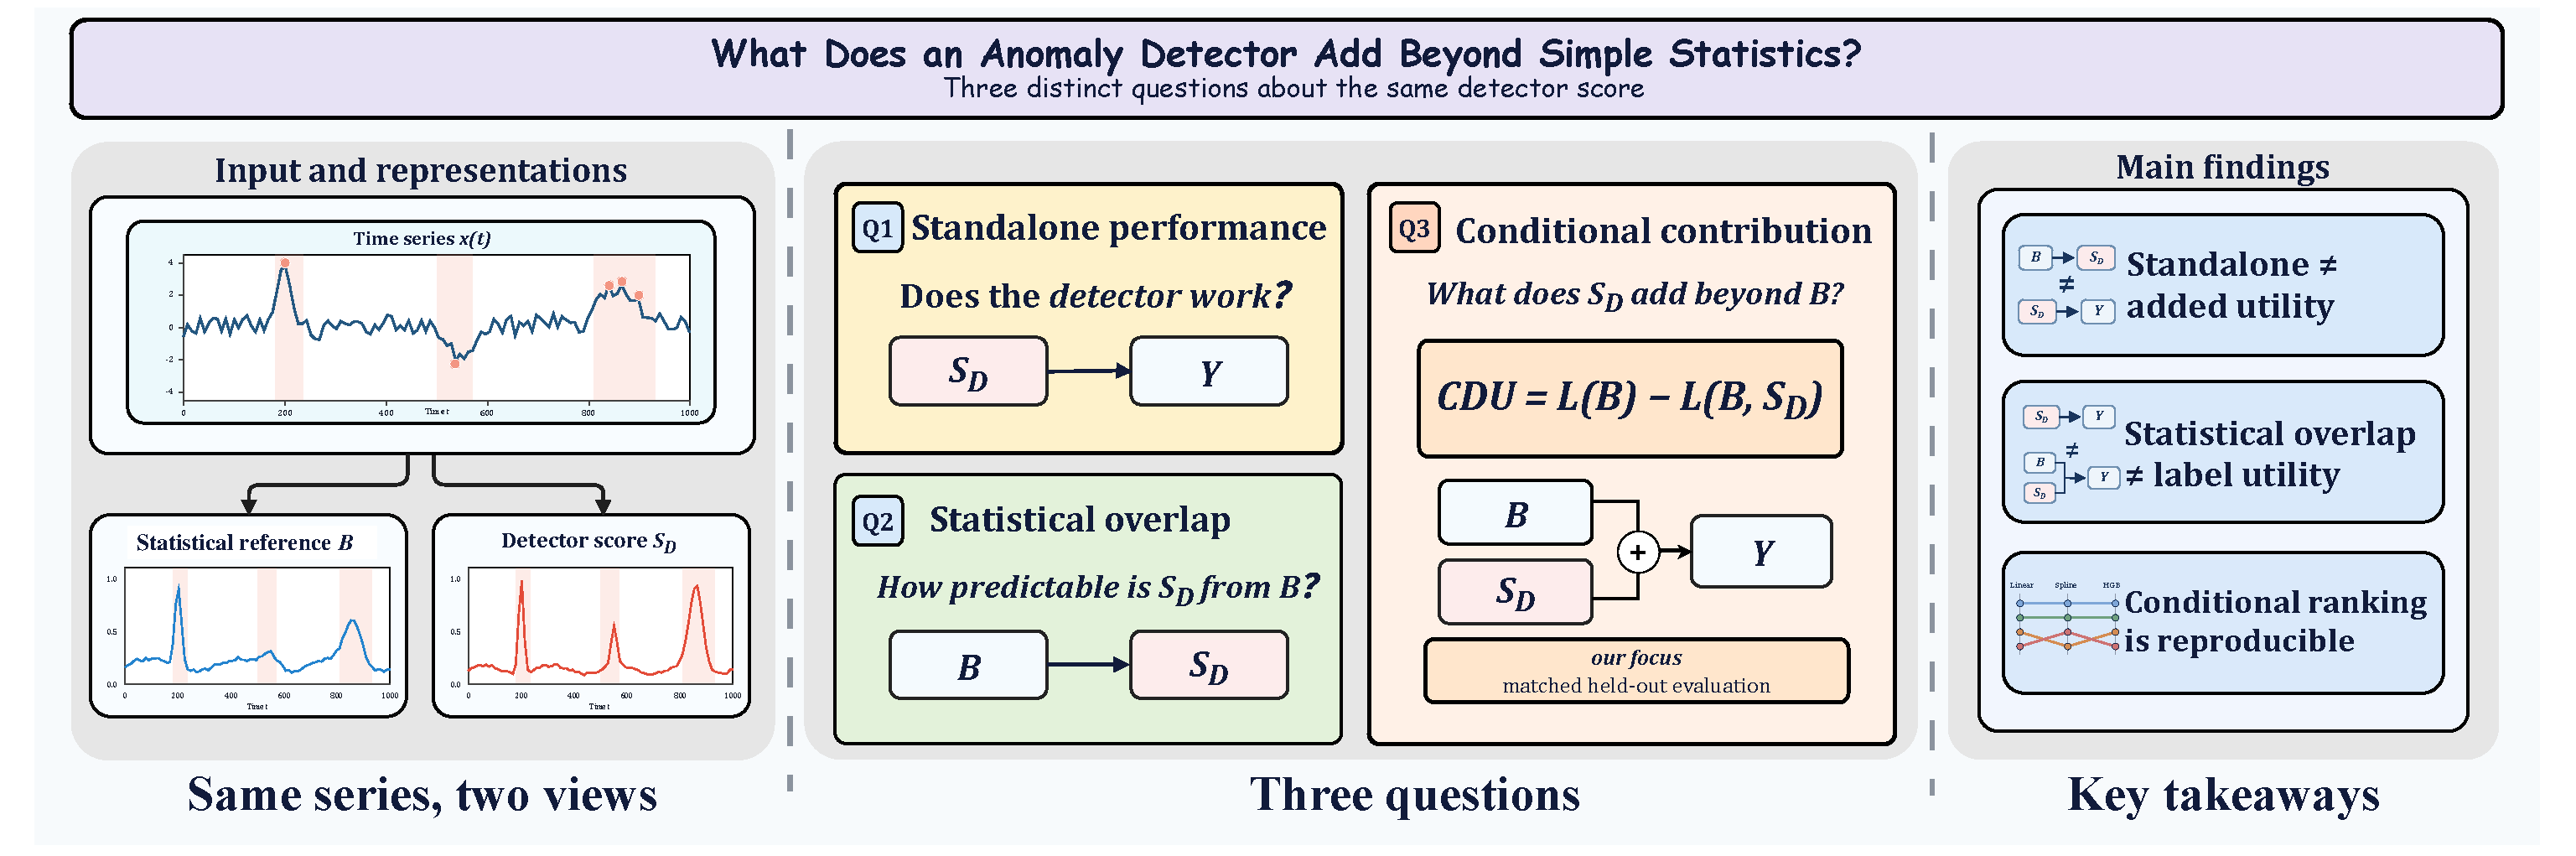
\includegraphics[width=\textwidth]{figures/main_concept.pdf}
\caption{The same series yields a statistical reference and a detector score. We distinguish standalone performance (Q1), statistical overlap (Q2), and conditional contribution (Q3); the three comparisons answer different questions.}
\label{fig:protocol}
\end{figure*}

\section{Conditional Detection Utility}
\subsection{Conditional detection utility}
Let $Y\in\{0,1\}$ denote an anomaly label, $B\in\mathbb R^p$ a statistical reference, and $S_D$ a detector score. For each held-out source, fit two probability predictors from the same probe family $\Probe$: one receives $B$, and the other $(B,S_D)$. Both use the same training points, weights, and fitting settings. The operational estimate is
\begin{equation}
\widehat{\mathrm{CDU}}_{\mathcal Q}(D\mid B)=\widehat L_B-\widehat L_{BD},
\label{eq:cdu}
\end{equation}
where $\widehat L_B$ and $\widehat L_{BD}$ are their paired held-out log-losses in bits. Positive CDU means that the detector improves label prediction given the reference. Figure~\ref{fig:protocol} summarizes the comparison.

For a matched standalone comparison, $U_D=\widehat L_0-\widehat L_D$, where the detector-only probe receives $S_D$ and the null uses training-source anomaly prevalence. Thus $U_D$ and CDU use the same loss but different reference information.

Define $\Risk^*(X)=\inf_q\E[-\log_2 q(Y\mid X)]$, where $q$ ranges over conditional probability distributions.\par\noindent\textbf{Proposition 1.} Under a common joint distribution and unrestricted predictors,
\begin{equation}
\begin{aligned}
\CDU^*(D\mid B)&=\Risk^*(B)-\Risk^*(B,S_D)\\
&=I(Y;S_D\mid B).
\end{aligned}
\end{equation}
\noindent\textit{Proof.} For any input $X$, the cross-entropy decomposition gives
\begin{equation}
\begin{aligned}
\E[-\log_2 q(Y\mid X)]&=H(Y\mid X)\\
&\quad+\E_X D_{\rm KL}(P_{Y\mid X}\Vert q_{Y\mid X}).
\end{aligned}
\end{equation}
The KL term is nonnegative and vanishes for the true conditional distribution, so $\Risk^*(X)=H(Y\mid X)$. Therefore,
\begin{equation}
\begin{aligned}
\Risk^*(B)-\Risk^*(B,S_D)
&=H(Y\mid B)-H(Y\mid B,S_D)\\
&=I(Y;S_D\mid B).
\end{aligned}
\end{equation}
This proves the identity.\hfill$\square$

Population CDU is nonnegative and vanishes when $Y\perp S_D\mid B$, including $S_D=g(B)$. Finite-probe CDU is predictor-family-relative and may be negative under transfer; it is not an exact estimate of conditional mutual information.

\subsection{Score interface}
Each curve is aligned to the same time indices as its labels. We evaluate within-series anomaly ordering through average ranks, removing detector-specific score spacing. For a length-$T_i$ curve, ranks start at one:
\begin{equation}
\widetilde s_{it}=\frac{\operatorname{rank}_{\rm avg}(s_{it})-0.5}{T_i}.
\end{equation}
The statistical reference uses the same rank representation. Ties are preserved, and constant curves map to 0.5. Rank normalization is part of the evaluation definition: it measures the label information added by a detector's anomaly ordering beyond the rank-normalized statistical reference. The transform is label-free; $B$ and $S_D$ below denote these probe inputs.

\subsection{Source-held-out estimation}
A source is a benchmark dataset group. Each outer fold excludes all series of one source from probe training. Labels from the remaining sources supervise the probes; held-out labels are used only to compute losses. Detector outputs and the statistical reference remain fixed. This strict split prevents probes from exploiting sibling series from the held-out source.

Let $G_{\rm tr}$ be the number of training sources and $n_g$ the number of series in training source $g$. If $m_i$ points are retained from series $i$ and $N_s=\sum_i m_i$, assign each retained point weight
\begin{equation}
w_{it}=\frac{N_s}{G_{\rm tr}n_gm_i}.
\end{equation}
This gives equal total weight to sources and to series within each source. Training retains $m_i=\min(T_i,2048)$ points per series; every test point is evaluated. A common basis-only predictor supplies the reference loss for all detectors within each fold. With binary log-loss $\ell$ and held-out probability $p_{it}^M$ for model $M$, aggregation is
\begin{equation}
\begin{aligned}
L_i^M&=\frac{1}{T_i}\sum_{t=1}^{T_i}\ell(y_{it},p_{it}^M),\\
\widehat L_M&=\frac{1}{G}\sum_{g=1}^{G}\frac{1}{n_g}\sum_{i\in g}L_i^M.
\end{aligned}
\end{equation}
Here $G=23$; paired source-bootstrap intervals quantify variation across held-out sources.

\begin{table*}[t]
\centering
\small
\caption{Primary spline results for nine fixed detector scores. VUS-PR is series-macro; $U_D$ and CDU are in bits. Parentheses give ranks; brackets give source-bootstrap 95\% intervals.}
\label{tab:main}
\setlength{\tabcolsep}{7pt}
\begin{tabular}{ccccc}
\toprule
Detector & VUS-PR (rank) & $U_D$ (rank) & CDU [95\% CI] & CDU rank \\
\midrule
SubPCA & 0.4224 (1) & 0.04060 (1) & 0.01509 [0.00256, 0.02964] & 1 \\
POLY & 0.3893 (2) & 0.02700 (3) & 0.00604 [0.00246, 0.00969] & 3 \\
MOMENT-FT & 0.3864 (3) & 0.01907 (4) & 0.00099 [-0.00001, 0.00208] & 7 \\
MOMENT-ZS & 0.3832 (4) & 0.01832 (5) & 0.00011 [-0.00088, 0.00113] & 9 \\
M2N2 & 0.2870 (5) & 0.03090 (2) & 0.01272 [0.00075, 0.02614] & 2 \\
TranAD & 0.2754 (6) & 0.01438 (6) & 0.00484 [-0.00162, 0.01263] & 4 \\
TimesNet & 0.2627 (7) & 0.00591 (8) & 0.00133 [-0.00015, 0.00300] & 5 \\
FITS & 0.2464 (8) & 0.00598 (7) & 0.00109 [-0.00008, 0.00221] & 6 \\
AnomalyTransformer & 0.1118 (9) & -0.00005 (9) & 0.00015 [-0.00129, 0.00167] & 8 \\
\bottomrule
\end{tabular}
\end{table*}

\begin{figure*}[!t]
\centering
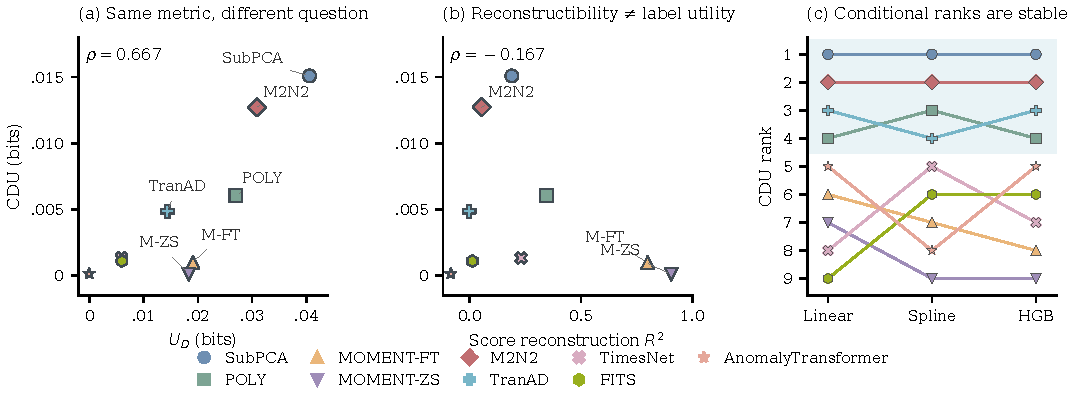
\includegraphics[width=\textwidth]{figures/conditional_comparison.pdf}
\caption{The benchmark blind spot and its consequences. (a) Detector-only and conditional utility use the same spline probe and log-loss yet differ; (b) statistical reconstructibility does not determine CDU; (c) the top-two order and top-four membership (shaded) persist across probes.}
\label{fig:intervals}
\end{figure*}

\section{Experimental Setup}
\label{sec:setup}
\textbf{Data and detectors.} We evaluate 350 univariate series from TSB-AD-U~\cite{liu2024tsbad}, following the evaluation population in~\cite{zhu2026oneliners}. Source groups follow the dataset identifier in each filename; MSL and SMAP are distinct, and UCR is grouped as one archive. We use SubPCA and POLY benchmark implementations~\cite{liu2024tsbad}, fine-tuned (FT) and zero-shot (ZS) MOMENT~\cite{goswami2024moment}, M2N2~\cite{kim2024m2n2}, TranAD~\cite{tuli2022tranad}, TimesNet~\cite{wu2023timesnet}, FITS~\cite{xu2024fits}, and AnomalyTransformer~\cite{xu2022anomaly}. All 350 curves are retained for every detector.

\textbf{Statistical reference.} The 31 fixed, label-free features span local variance, range, prediction deviation, absolute difference, robust dispersion, and spectral entropy. No feature is selected using held-out labels.

\textbf{Probes and comparisons.} Additive cubic-spline logistic regression is the primary probe; linear logistic and histogram gradient boosting (HGB) test probe sensitivity. All use the same label-independent training sample (at most 2048 points per series), source/series weights, and full test curves. Logistic probes use $C=0.1$, spline has four fixed knots, and HGB runs for 32 iterations. VUS-PR and CDU use the same detector curves.

\textbf{Reconstruction and robustness.} Source-held-out ridge regression predicts ranked detector scores from $B$ ($\alpha=1$); we report source-macro $R^2$ and Spearman correlation. We repeat the spline comparison across five sampling seeds, seven reference-family removals, cumulative 7--29-feature references, and alternative detector-score interfaces (min--max or Gaussianized z-scores).

\textbf{Controls.} We test a duplicated reference feature, independent Gaussian noise, and a synthetic score $Z+2Y$ with independent $Z\sim\mathcal N(0,1)$. Only the last control uses labels.

\section{Results and Interpretation}
\subsection{Standalone performance and added utility tell different stories}
Table~\ref{tab:main} and Fig.~\ref{fig:intervals}a compare detector-only utility $U_D$ with CDU under the same spline probe, log-loss, held-out sources, and weights. MOMENT-FT and MOMENT-ZS fall from $U_D$ ranks 4 and 5 to CDU ranks 7 and 9, while TranAD rises from 6 to 4. Across linear, spline, and HGB probes, the $U_D$/CDU rank correlations are 0.967, 0.667, and 0.500. The distinction also appears alongside benchmark VUS-PR: M2N2 and TranAD move from VUS ranks 5 and 6 to CDU ranks 2 and 4.

POLY and both MOMENT variants have similar VUS-PR (0.3832--0.3893), yet POLY exceeds MOMENT-FT by 0.00505 bits of spline CDU [0.00172, 0.00860] and MOMENT-ZS by 0.00593 [0.00241, 0.00961]. Both differences remain positive after a joint max-standardized bootstrap correction over three pairwise POLY/MOMENT comparisons across the three probes.

\subsection{Score reconstructibility does not determine added label utility}
Source-held-out ridge regression reconstructs MOMENT-FT and MOMENT-ZS scores strongly (source-macro $R^2=0.799$ and 0.904; Spearman 0.895 and 0.951), but M2N2 and TranAD weakly ($R^2=0.054$ and $-0.002$). Across nine detectors, reconstruction $R^2$ and spline CDU have Spearman correlation $-0.167$ (Fig.~\ref{fig:intervals}b). Statistical overlap and added label utility show little alignment in this detector set: a hard-to-reconstruct score helps only if its residual information improves label prediction.

\subsection{The conditional comparison is reproducible}
SubPCA and M2N2 remain first and second across linear, spline, and HGB; TranAD and POLY complete the same top-four set (Fig.~\ref{fig:intervals}c). Pairwise rank correlations are 0.717--0.867. Spline and HGB extract substantially more predictive signal from the statistical reference than linear logistic: their basis losses are 0.2891 and 0.2869 bits versus 0.3375. Expanding linear training from sampled to full points barely changes basis loss (0.337462 versus 0.337447), indicating that the gap is driven by probe expressivity rather than additional training points.

Five training-sampling seeds give identical spline ranks. Seven reference-family removals yield rank correlations of 0.917--1.000; cumulative references with 7--29 features retain the full-reference top four ($\rho=0.933$--1.000). A Gaussian-CDF-transformed z-score interface also retains that group ($\rho=0.933$). Min--max scaling preserves detector-specific score spacing and changes the broader ranking ($\rho=0.517$), moving POLY from rank 3 to 9. This contrast motivates the common rank interface: our primary CDU comparison concerns anomaly ordering rather than detector-specific score geometry.

\subsection{Controls validate the intended behavior}
Matched duplicate and independent-noise controls remain near zero, with no negative-control interval entirely above zero. Every label-informed synthetic control is clearly positive; spline synthetic CDU is 0.09220 bits [0.06819, 0.11712]. CDU separates redundant and irrelevant scores from complementary label signal.


\section{Discussion and Conclusion}
Complex TSAD detectors can perform well while overlapping strongly with simple statistical structure. Standalone performance, statistical overlap, and conditional contribution give different views of the same score; CDU quantifies the third. Across nine detectors, the conditional ranking differs from standalone evaluation and remains broadly consistent across probes, seeds, and reference variants. Reporting these views together clarifies what a detector adds beyond the fixed statistics.

Such comparisons may inform detector selection: models with similar standalone performance need not be interchangeable once their conditional contributions are measured. Using reference-relative utility to guide model combination or representation learning remains future work.

{\footnotesize\noindent\textbf{Acknowledgment.} OpenAI Codex was used for language and clarity editing. The authors reviewed and verified the final manuscript.\par}
